\documentclass[main.tex]{subfiles}

\begin{document}
\sloppy


\vspace{1.0cm}

\section{Implementazione di nuove funzionalità alle fixtures}\label{sec:NewFeatures}
Una volta creata una pipeline di rendering, sistemata la gerarchia dei componenti e fatta funzionare l'interpolazione è possibile finalmente aggiungere nuove features alle fixture virtuali. Come visto nel capitolo \ref{sec:RenderingPipeline}, per aggiungere una nuova feature bisogna:
\begin{itemize}
	\item Implementarla come codice HLSL
	\item Implementarla come MaterialFunction
	\item Aggiungerla al generatore di codice HLSL
	\item Aggiungerla al generatore della pipeline per il rendering del materiale Light e Lens
\end{itemize}
In questo capitolo non tratteremo mai il secondo punto poiché rappresenta la trasposizione in MaterialExpression del codice già visto in HLSL.

\subsection{Sagomatori}\label{subsec:5_shaper}
Il sistema dei sagomatori (detto anche \say{framing system} oppure \say{shaper}) consiste in un modulo composto da 4 lame (dette anche \say{bandiere}) che possono immettersi ed inclinasi singolarmente all'interno del fascio di luce. Inoltre, l'intero modulo può roteare, muovendo contemporaneamente la direzione in cui si immettono tutte le lame si immettono.
%TODO Esempi con foto
Il controllo della lama può avvenie in due modi:
\begin{itemize}
	\item \textbf{A+B}: Controlliamo singolarmente l'immissione dei due punti estremi della lama ($A$ e $B$). Per avere la lama \say{dritta} Dovremmo avere $A = B$, per inclinarla da un lato basta avere uno dei due valori maggiori dell'altro.
	\item \textbf{A+Rot}: Controlliamo l'immissione della lama ($A$) e separatamente la sua inclinazione ($R$).
\end{itemize}
\begin{figure}[H]
    \centering
    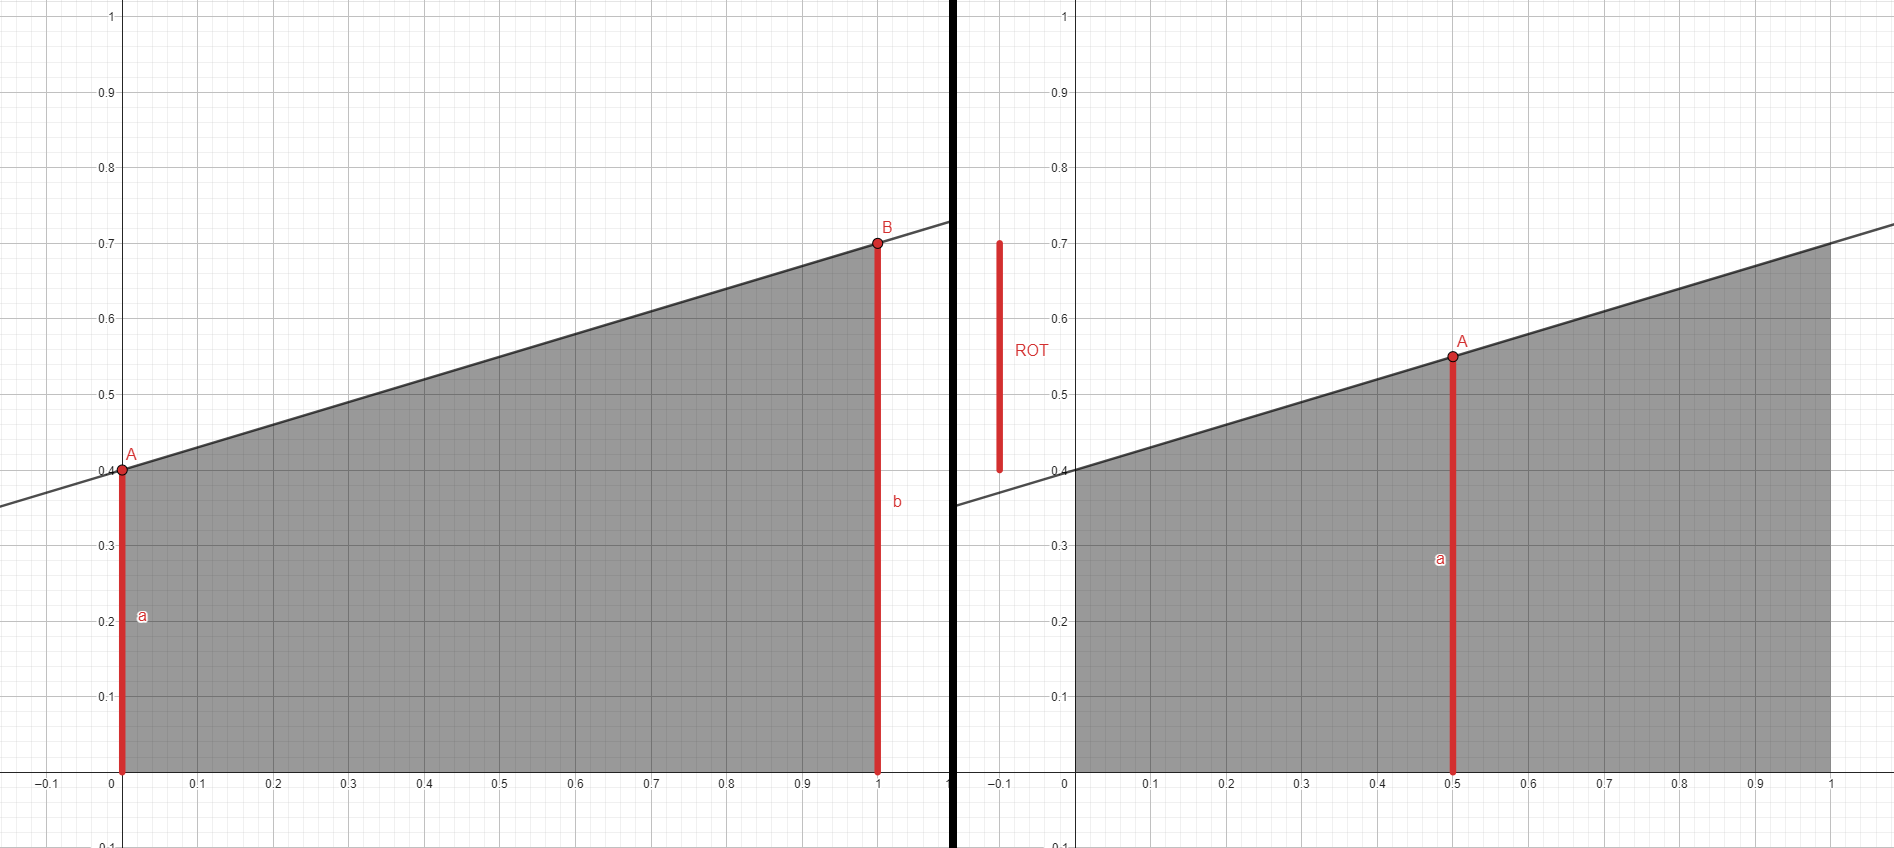
\includegraphics[width=1\linewidth]{img/newFeatures/abVSarot.png}
    \caption{A sinistra, la modalità di controllo \textit{A+B}. A destra, \textit{A+Rot}}
    \label{fig:5_shaperFixes}
\end{figure}

Effettuare il rendering di una funzionalità come lo shaper attraverso texture è davvero oneroso in termini computazionali. La scelta migliore è fare il rendering immaginandoci il framing system come delle equazioni matematiche. In generale, il rendering di un material avviene effettuando il rendering di varie coordinate UV, ovvero coordinate bidimensionali normalizzate tra [0, 1]. Possiamo immaginare il nostro codice come se fosse inserito in un ciclo for che si scorre \say{tutte} le x e le y comprese tra 0 ed 1. Il nostro codice però si occupa di renderizzare una sola UV alla volta. 

\subsubsection{Idea come formula matematica}\label{subsec:5_1_ShaperMath}
\begin{wrapfigure}{r}{0.45\textwidth}
    \centering
    \captionsetup{justification=centering}
    
\includegraphics[scale=0.35]{img/newFeatures/eqExample.jpg}
    \caption{Esempio di rendering con il codice \lstinline{return y > 0.5;}}
    \label{fig:5_eqExample}
\end{wrapfigure}
Se immaginiamo quindi una singola lama come una equazione matematica, possiamo renderizzarla controllando semplicemente se la Y della coordinata UV che stiamo renderizzando in quel momento si trova sopra o sotto l'equazione. Il nostro lavoro diventa quindi generare la corretta equazione matematica in base agli input $A$ e $B$ o $R$.

Per trovare l'equazione della retta quando facciamo il sample A+B, possiamo ricorrere alla formula per ottenere l'equazione di una retta passante per due punti:
\[m = \frac{y_2 - y_1}{x_2 - x_1}\]
Immaginiamo che i valori di $A$ e $B$ corrispondano alle loro y, che $A$ si trovi a coordinate $x = 0$ e che $B$ si trovi a $x = 1$. La formula sarà uguale a
\[m = \frac{y_B - y_A}{x_B - x_A} = \frac{B - A}{1 - 0} = B - A\]
In questo modo generiamo il coefficiente una retta che però ha sempre origine in $(0, 0)$. Nella realtà, ciò che abbiamo appena creato è una bandiare in cui solamente il valore B \say{funziona}. Per far \say{funzionare} anche il valore $A$, basta aggiungerlo come termine noto del'equazione. Come scritto sopra, per generare una flag bisogna controllare quando stiamo \say{sopra} questa equazione, rendendola quindi uguale a:
\[y > x(B - A) + A\]
\newline

Per effettuare, invece, il sampling di una flag A+Rot, possiamo utilizzare $A$ come termine noto, e convertire $R$ da gradi alla relativa tangente trigonometrica in modo da avere direttamente il coefficiente della retta. Poiché vogliamo però inclinare questa retta usando come punto di rotazione il suo centro ($x = 0.5$) e non la sua origine ($x = 0$), dobbiamo modificare il termine noto in base al coefficiente: più il coefficiente zè elevato (e più la retta sarà quindi inclinata crescendo da sinistra verso destra) e più il termine noto dovrà calare. Considerando la sezione della retta compresa tra $x = [0, 1]$, la tangente di $R$, essendo direttamente uguale al coefficiente della retta, è anche uguale alla differenza tra il valore della $y$ quando la retta avrà $x = 0$ e quando avrà $x = 1$. Al centro di questa sezione (quando $x = 0.5$) la differenza con i due estremi sarà quindi uguale a $\frac{tan(R)}{2}$, ovvero esattamente il valore da sottrarre al termine noto per mantenere centrale il punto di rotazione della retta. La formula finale dell'equazione sarà quindi:
\[y > tan(R)x + (a - \frac{tan(R)}{2})\]

Come anche le ruote, anche il framing system deve implementare il frost. Piuttosto di applicare un filtro di blur al framing system già renderizzato, è preferibile in termini di peso computazionale implementare una sfocatura come formula matematica direttamente nel precedente rendering. L'idea è quella di utilizzare il valore del frost per definire la dimensione di una zona di sfumatura intorno alla retta. La prima operazione che viene effettuata è trovare la distanza della coordinata UV che stiamo renderizzando dalla retta. Questa operazione viene approssimata come la distanza assoluta ($d$) tra la $y$ della coordinata UV e la $y$ della retta per ogni $x$.
\[d = \abs{y - g(x)}\]
Dove $g(x)$ è la funzione matematica scelta per effettuare il sample della flag.

Lo step suguente è trasformare il valore di frost ($f$) dentro una semplice funzione di remapping:
\[remapFrost(f) \coloneqq f * 0.05 + 0.002\]
Dove $0.05$ e $0.002$ sono valori magici trovati dopo discreti tentativi di try and error.

Successivamente viene applicata un'altra funzione di remapping sulla distanza, in modo che sia scalata all'interno del valore frost:
\[remapDist(d, f) \coloneqq 
	\begin{dcases}
		\hfil 1 & \text{se } d > remapFrost(f)\\
		\frac{d}{remapFrost(f)} & \text{altrimenti}
	\end{dcases}
\]

Poiché $d$ all'inizio viene calcolata come distanza assoluta dalla retta, con quanto definito fin'ora avremo una figura nera si dissolve andando verso il bianco quando siamo abbastanza vicini alla retta stessa. Dobbiamo invece fare in modo che la dissolvenza parta da bianco, diventi grigia in corrispondenza della retta, e nera dopo la stessa:
\[fade(d, f) \coloneqq 
	\begin{dcases}
		\hfil	 \frac{remapDist(d, f)}{2} & \text{se } y > g(x)\\
				-\frac{remapDist(d, f)}{2} & \text{altrimenti}
	\end{dcases}
\]
\newline

\begin{wrapfigure}{r}{0.45\textwidth}
    \centering
    \captionsetup{justification=centering}
    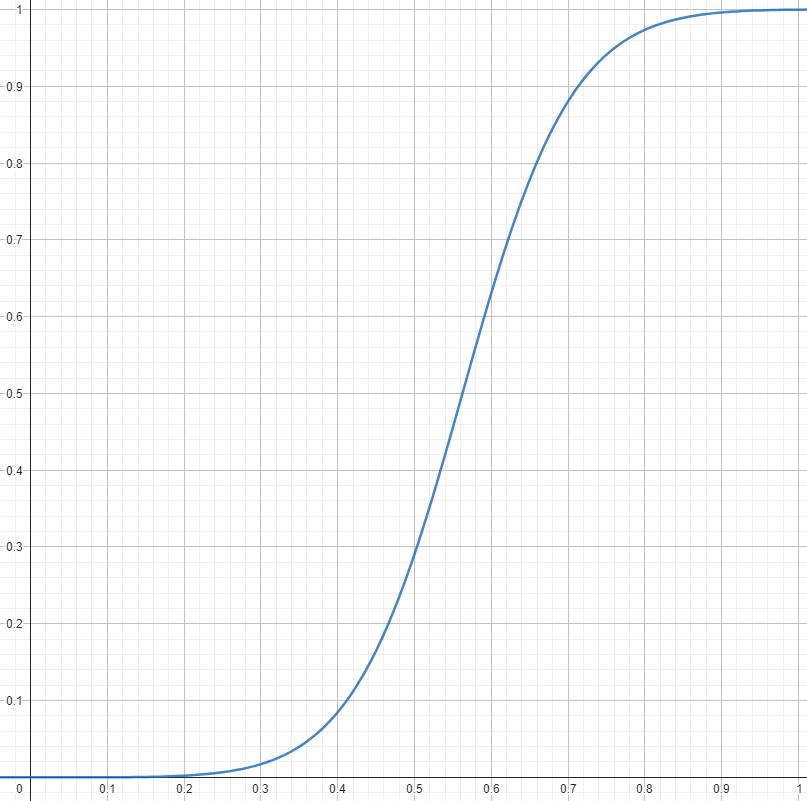
\includegraphics[scale=0.35]{img/newFeatures/sCurve.png}
    \caption{Funzione $sCurve(v)$}
    \label{fig:5_sCurve}
\end{wrapfigure}
Per un effetto ottico in cui è molto più semplice distinguere gradazioni differenti di colori scuri rispetto a gradazioni differenti di colori chiari, applicando il frost sembrerà che la sagomatura si sposti verso il basso, come in figura \ref{fig:5_shaperFixes}. Per compensare ciò, il risultato finale calcolato in precedenza, viene passato all'interno di un'ultima funzione di remapping: quello che vogliamo è creare una curva ad S (figura \ref{fig:5_sCurve}), in modo che la dissolvenza avvenga repentinamente al centro dei nostri valori piuttosto che linearmente da 0 ad 1.
\[sCurve(v) \coloneqq \frac{1}{1 + (\frac{v}{1.125 - v})^{-4}}\]
Dove i valori all'interno della frazione e l'esponenziale sono ottenuti via try ed error. Il valore $1.125$ serve per sbilanciare verso destra la curva, l'esponenziale per regolarne l'ampiezza.
\begin{figure}[H]
    \centering
    
\includegraphics[width=1\linewidth]{img/newFeatures/shaperFixes.jpg}
    \caption{Da destra verso sinistra: flag senza frost, flag con frost e passaggio dei valori lineare tra 0 ed 1, flag con frost e con la funzione $sCurve(v)$ applicata.}
    \label{fig:5_shaperFixes}
\end{figure}


Con il frost abilitato si verifica anche un altro problema: Quando una flag è completamente aperta oppure è completamente chiusa, vedremo comunque renderizzata la sfumatura del frost. Le fixture reali risolvono questo problema facendo muovere le bandiere oltre i limiti di apertura e chiusura. Creiamo quindi una funzione da anteporre a tutti i calcoli per questa feature, che modifichi il valore di $A$ e di $B$. 
\[frostLimit(f) \coloneqq 
	\begin{dcases}
		\hfil f & \text{se } f < 0.2\\
		0.2 & \text{altrimenti}
	\end{dcases}
\]
\[remapABposition(x, f) \coloneqq x(2 * frostLimit(f) + 1) - frostLimit(f)\]
% x = max(frost, 0.2)
% res = (inp * (x * 2 + 1)) - x
Questa funzione si occupa di rimappare il valore di $A$ o di $B$ all'interno di un range più piccolo, al variare del valore di frost. Questa rimapperà tutti i valori in un range via via più piccolo man mano che cresce il valore di frost. Viene anche imposto un valore minimo di frost, in modo da emulare l'effetto della lama che supera i limiti di apertura e chiusura anche quando è disattivato.
\newline

La direzione di ogni singola bandiera, così come la rotazione dell'intero framing system viene implementata come un'unica funzione \cite{UVrotation} che prende in input la somma dei due valori:
\[finalAngle = direction + framingSystemAngle\]
Dove $direction$ può essere uguale a 0, 90, 180 o 270 gradi. La rotazione viene effettuata trasformando i valori UV prima di qualsiasi altro calcolo effettuato per il sample di ogni singola blade.
\[rotateUV(a) \coloneqq 
	\begin{bmatrix}
		cos(a)(x - \frac{1}{2}) + sin(a)(y - \frac{1}{2}) + x \\
		cos(a)(y - \frac{1}{2}) + sin(a)(x - \frac{1}{2}) + y
	\end{bmatrix}
\]
Dove $a$ corrisponde ai gradi di rotazione in input.

\subsubsection{Generazione codice HLSL ed inserimento nel materiale Beam}\label{subsec:5_1_ShaperHlsl}
\lstset{language=glsl}
Le funzioni $fade$, $sCurve$ e $rotateUV$ sono state scritte in maniera generica poiché sono utili anche nel sample di altre features (Ad esempio, l'iris \ref{subsec:5_Iris}). Le funzioni di remapping sono state, invece, accorpate tra di loro. Le condizioni sono implementate con la formula \lstinline{float b = /*boolean expression*/; float f = b * x + (1 - b) * y;} per ridurre la branch divergence nell'esecuzione del codice hlsl.
\begin{lstlisting}
float sCurve(float f){
	const float exp = -4;
	f = saturate(f);
	return 1 / (1 + pow((f / (1.125 - f)), exp));
}

void rotateUV(float2 texCoor, float rads, out float x, out float y) {
	float c = cos(rads);
	float s = sin(rads);
	x = c * (texCoor.x - 0.5) + s * (texCoor.y - 0.5) + 0.5;
	y = s * (texCoor.x - 0.5) - c * (texCoor.y - 0.5) + 0.5;
}

float fade(float passed, float d, float frost, float frostMultiplier){
	float max = (0.05 * frost + 0.002) * frostMultiplier;
	float clamp = d > max;
	d = clamp + (1 - clamp) * (d / max);

	return sCurve((passed * 2 - 1) * (d / 2) + 0.5);
}
\end{lstlisting}

Il codice per fare il sample delle due differenti modalità è implementato come due funzioni separate, seppur molto simili:
\begin{lstlisting}
float sampleBladeAB(float2 texCoor, float a, float b,
		float orientationRads, float frost){
	float x, y;
	rotateUV(texCoor, orientationRads, x, y);
	float m = b - a;
	float eq = (x * m) + a;
	float d = abs(y - eq);
	float passed = y > eq;
	return mapLineValue(passed, d, frost, 1);
}
float sampleBladeARot(float2 texCoor, float a, float rotRads,
		float orientationRads, float frost){
	float x, y;
	rotateUV(texCoor, orientationRads, x, y);
	float m = rotRads * x;
	float eq = m - (rotRads * 0.5) + a;
	float d = abs(y - eq);
	float passed = y > eq;
	return mapLineValue(passed, d, frost, 1);
}
\end{lstlisting}


Il codice per la generazione del codice HLSL in se è molto semplice. Si prende in input un array di ShaperFixtureComponent già instanziati e per ciascuno controlla se sono in modalità A+B oppure A+Rot, e seleziona la relativa chiamata a funzione corretta.
\lstset{language=UEcpp}
\begin{lstlisting}
for (int i = 0; i < mShapers.Num(); i++) {
    FString orientationVarName =
        CPGDTFRenderPipelineBuilder::getInputBladeOrientationName(
            mShapers[i]->getOrientation()
        );
    FString bRotVarName =
        CPGDTFRenderPipelineBuilder::getInputBladeABRotName(
            false, mShapers[i]->getOrientation()
        );
    FString aVarName =
        CPGDTFRenderPipelineBuilder::getInputBladeABRotName(
            true, mShapers[i]->getOrientation()
        );

    if (mShapers[i]->isInAbMode()) { //a+b mode
        placeholderCode = placeholderCode + FString::Format(*textAdd, {
            FString::Printf(
                TEXT("sampleBladeAB(pos.xy, %s, %s, %s, %s)"),
            *aVarName, *bRotVarName, *orientationVarName, *frostVarName)
        });
    } else { //a + rot mode
        placeholderCode = placeholderCode + FString::Format(*textAdd, {
            FString::Printf(
                TEXT("sampleBladeARot(pos.xy, %s, %s, %s, %s)"),
            *aVarName, *bRotVarName, *orientationVarName, *frostVarName)
        });
    }
}
\end{lstlisting}

La funzione $remapABposition$ è stata implementata come MaterialFunction invece che come codice hlsl, in modo che possa venire ottimizzata automaticamente da UnrealEngine \cite{hlslNoOptimize}. Inoltre è stata creata un'altra MaterialFunction (ConvertRot) che si occupa di convertire i gradi in radianti e di ottenerne il valore della tangente. L'inserimento degli input e dei parametri nel materiale Beam inizia caricandosi queste due MaterialFunction.
\begin{lstlisting}
UMaterialFunctionInterface* mfShaperConvertBladePosition =
    Cast<UMaterialFunctionInterface>(
        FCPGDTFImporterUtils::LoadObjectByPath(
            mfShaperConvertBladePositionPath
        )
    );
UMaterialFunctionInterface* mfShaperConvertRot =
    Cast<UMaterialFunctionInterface>(
        FCPGDTFImporterUtils::LoadObjectByPath(
            mfShaperConvertRotPath
        )
    );
\end{lstlisting}
Successivamente viene creata una lambda che si occuperà di aggiungere effettivamente un parametro al materiale.
\begin{lstlisting}
const std::function<void(FString, FString, bool)>
    addABRotParameterToBeamPipeline = [&](
        FString paramName, //Nome del parametro del materiale
        FString variableName, //Nome della variabile della CE
        bool isRot //Se true, il parametro corrisponde al valore "rot"
    ) {
    //...
}
\end{lstlisting}
Infine si scorre la lista degli shaper e per ciascuno aggiunge tre parametri, A, B/Rot e rotazione. Quando viene generato il parametro B/Rot si controlla la modalità dello shaper attraverso la funzione \lstinline{isInAbMode()}.
\begin{lstlisting}
for (UCPGDTFShaperFixtureComponent *shaper : shapers) {
    int orientation = shaper->getOrientation(); //ID della flag

    addABRotParameterToBeamPipeline( //Generazione parametro A
        getBladeABRotParamName(true, orientation),
        getInputBladeABRotName(true, orientation),
        false
    );
    addABRotParameterToBeamPipeline( //Generazione parametro B/Rot
        getBladeABRotParamName(false, orientation),
        getInputBladeABRotName(false, orientation),
        !shaper->isInAbMode()
    );
    addScalarInputToBeamPipeline( //Parametro per la rotazione
        dstMaterial,
        getBladeOrientationParamName(orientation),
        getInputBladeOrientationName(orientation),
        meCustom, meBlocksMover
    );
}
\end{lstlisting}
Dove \lstinline{getBladeABRotParamName()} e \lstinline{getInputBladeABRotName()} prendono \lstinline{true} se stiamo generando il parametro A o \lstinline{false} se stiamo generando il parametro B o Rot (I due valori condividono lo stesso parametro). \newline

La lambda citata sopra si occupa come prima cosa di generare il parametro effettivo.
\begin{lstlisting}
    UMaterialExpressionScalarParameter* param =
        generateMaterialExpression<UMaterialExpressionScalarParameter>(
            dstMaterial
        );
    param->ParameterName = FName(*paramName);
    param->Group = FName(TEXT("Runtime Parameters"));
    param->SortPriority = 5;
    param->DefaultValue = 0;
    dstMaterial->GetEditorOnlyData()->ExpressionCollection.
        AddExpression(param);
\end{lstlisting}
Successivamente crea, imposta, collega e sposta la MaterialFunctionCall in base alla modalità selezionata.
\begin{lstlisting}
UMaterialExpressionMaterialFunctionCall* mfCall = 
    generateMaterialExpression<UMaterialExpressionMaterialFunctionCall>(
        dstMaterial
    );
dstMaterial->GetEditorOnlyData()->ExpressionCollection.
    AddExpression(mfCall);
if (isRot) {
    mfCall->SetMaterialFunction(mfShaperConvertRot);
} else {
    mfCall->SetMaterialFunction(mfShaperConvertBladePosition);
    mfCall->FunctionInputs[1].Input.Connect(0, scalarFrost); //Frost
}
mfCall->FunctionInputs[0].Input.Connect(0, param); //Value

mfCall->MaterialExpressionEditorX =
    meBlocksMover->getCurrentX()+ BEAM_EDITOR_BLOCK_DISTANCE_X;
mfCall->MaterialExpressionEditorY =
    meBlocksMover->getCurrentY() + EDITOR_MINI_BLOCK_SIZE;
meBlocksMover->moveMaterialExpression(param, EDITOR_SCALAR_PARAM_SIZE);
\end{lstlisting}
Infine, genera un input sulla CustomExpression e lo collega alla precedente MaterialFunctionCall.
\begin{lstlisting}
FCustomInput input;
input.InputName = FName(*variableName);
input.Input.Connect(0, mfCall);
meCustom->Inputs.Add(input);
\end{lstlisting}

\subsubsection{Generazione nella RenderingPipeline per Light e Lens}\label{subsec:5_1_ShaperRenderingPipeline}
Come per la generazione del materiale Beam anche qui le varie funzioni descritte nel capitolo \ref{subsec:5_1_ShaperMath} sono state trasformate in MaterialFunctions. Come spiegato nella sezione \ref{sec:RenderingPipeline} tali MaterialFunctions prenderanno in input l'output della precedente, per formare la pipeline di rendering. L'implementazione in se delle MaterialFunctions non viene vista poiché è identica al codice HLSL spiegato nel capitolo precedente, bensì vedremo comunque la parte di generazione della pipeline. \newline

Si effettua un ciclo su tutti gli ShaperFixtureComponent che dobbiamo aggiungere alla pipeline. Per ciascuno, iniziamo con lo generare una MaterialFunctionCall ed impostarne la MaterialFunction in base alla modalità della flag.
\begin{lstlisting}
int orientation = shaper->getOrientation();
UMaterialExpressionMaterialFunctionCall* currentNode =
    generateMaterialExpression<UMaterialExpressionMaterialFunctionCall>(
        dstMaterial
    );
dstMaterialData->ExpressionCollection.AddExpression(currentNode);

if (shaper->isInAbMode()) currentNode->SetMaterialFunction(mfShaperAB);
    else currentNode->SetMaterialFunction(mfShaperARot);
\end{lstlisting}
Successivamente vengono generati e connessi i vari parametri della precedente MaterialFunctionCall.
\begin{lstlisting}
auto aParam = addScalarParameterToMiPipeline(
    dstMaterial,
    getBladeABRotParamName(true, orientation),
    meParamsMover
);
auto bRotParam = addScalarParameterToMiPipeline(
    dstMaterial,
    getBladeABRotParamName(false, orientation),
    meParamsMover
);
auto orientationParam = addScalarParameterToMiPipeline
    dstMaterial,
    getBladeOrientationParamName(orientation),
    meParamsMover
);

currentNode->FunctionInputs[1].Input.Connect(0, previousParameter);
currentNode->FunctionInputs[2].Input.Connect(0, frostParam);
currentNode->FunctionInputs[3].Input.Connect(0, aParam);
currentNode->FunctionInputs[4].Input.Connect(0, bRotParam);
currentNode->FunctionInputs[5].Input.Connect(0, orientationParam);
\end{lstlisting}
Ed infine viene spostata ed impostata come ultimo nodo generato.
\begin{lstlisting}
meModulesMover->moveMaterialExpression(currentNode);
previousParameter = currentNode;
delete meParamsMover;
\end{lstlisting}

\subsubsection{ShaperFixtureComponent}\label{subsec:5_1_ShaperFixtureComponent}
L'implementazione del componente è molto semplice, vista la gerarchia dei componenti che abbiamo creato in precedenza. L'unico codice elaborato presente nel componente si trova nella funzione \lstinline{Setup()}, e si occupa solamente di capire in che modalità il componente viene usato. 

Questa operazione viene effettuata scorrendo tutta la lista di ChannelFunction assegnate al componente, e viene impostata la modalità \say{A+B} ogni qualvolta si incontra un componente B, oppure la modalità \say{A+Rot} ogni qualvolta si incontra un componente Rot.
\begin{lstlisting}
for (Per ogni ChannelFunction cf) {
    auto attrType =
        CPGDTFDescription::GetGDTFAttributeTypeValueFromString(
            cf.Attribute.Name.ToString()
        );

    if (attrType == ECPGDTFAttributeType::Blade_n_Rot) {
        abMode = false;
    } else if (
               attrType == ECPGDTFAttributeType::Blade_n_B
            || attrType == ECPGDTFAttributeType::BladeSoft_n_B
            ) {
        abMode = true;
    }
}
\end{lstlisting}

Di seguito, degli screenshot della classe per mostrare quanto sia semplice implementare nuovi componenti ora che la gerarchia di FixtureComponent è stata rivoluzionata.
\begin{figure}[H]
    \centering
    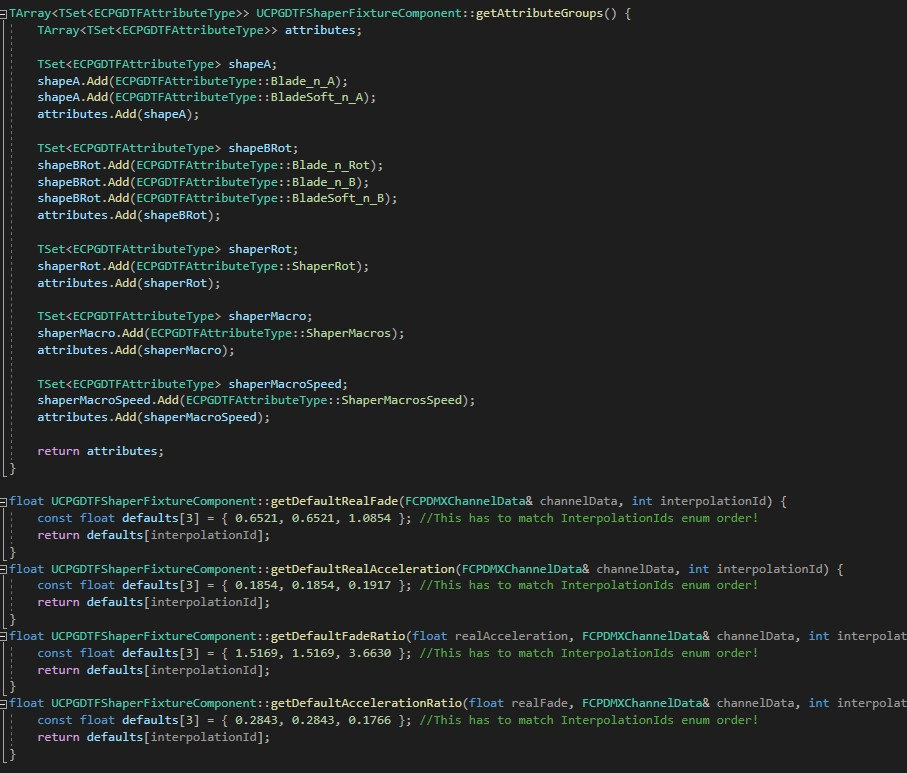
\includegraphics[width=1\linewidth]{img/newFeatures/ShaperComponentCode1.jpg}
    \label{fig:5_ShaperComponentCode1}
\end{figure}
\begin{figure}[H]
    \centering
    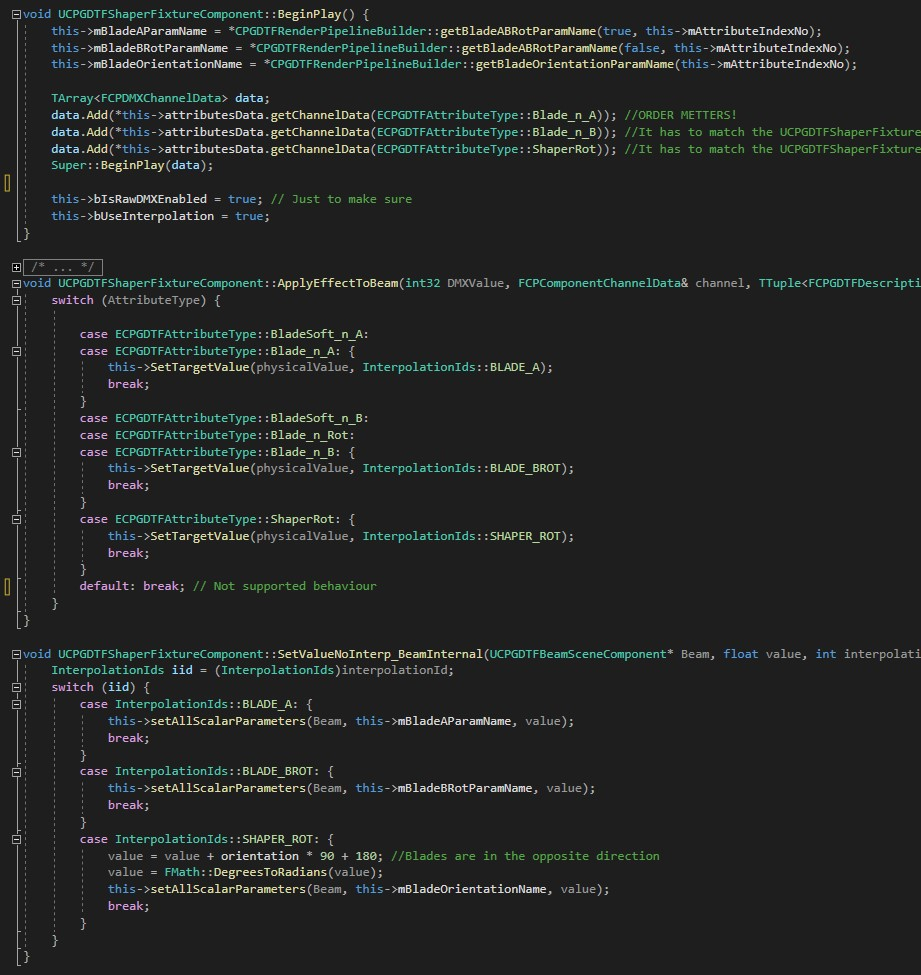
\includegraphics[width=1\linewidth]{img/newFeatures/ShaperComponentCode2.jpg}
    \label{fig:5_ShaperComponentCode2}
\end{figure}


\subsection{Iris}\label{subsec:5_Iris}

\subsubsection{Idea come formula matematica}\label{subsec:5_2_IrisMath}

\subsubsection{Generazione codice HLSL}\label{subsec:5_2_IrisHlsl}

\subsubsection{Generazione nella RenderingPipeline}\label{subsec:5_2_IrisRenderingPipeline}

\subsubsection{IrisFixtureComponent}\label{subsec:5_1_IrisFixtureComponent}

\end{document}